
スタンダードモード用入力ファイルは次のような格好をしています。

\begin{minipage}{10cm}
\begin{screen}
\begin{verbatim}
W = 2
 L = 4
 model = "spin"
 method = "Lanczos"

 lattice = "triangular lattice"
//mu = 1.0
// t = -1.0
// t' = -0.5
// U = 8.0
//V = 4.0
//V'=2.0
J = -1.0
J'=-0.5
// nelec = 8
2Sz = 0
\end{verbatim}
\end{screen}
\end{minipage}

大まかなルールは次のとおりです。
\begin{itemize}
\item 各行にはひと組ずつキーワード(\verb|=|の前)と
  パラメーター(\verb|=|の後)が書かれており間は\verb|=|で区切られています。
\item 各キーワードは順不同に記述できます。
\item 空白行、または\verb|//|で始まる行(コメントアウト)は読み飛ばされます。
\item 各キーワード、パラメーターの大文字$\cdot$小文字は区別されません。
  ダブルクオート、空白は無視されます。
\item 必ず指定しなければいけないパラメーター、
  指定しない場合デフォルト値が使われるパラメーター、
  (他のパラメーターの組み合わせによっては)使われないパラメーターが存在します。
  使われないパラメーターが指定された場合にはプログラムは終了し、
  入力ファイルをチェックするようにというメッセージが表示されます。
\end{itemize}

次に各キーワードの説明をします。

\subsection{計算の種類に関する必須パラメーター}

\begin{itemize}

\item \verb|model|

{\bf 形式 :} 文字列(\verb|"Fermion Hubbard"|, \verb|"Spin"|, \verb|"Kondo Lattice"|, 
\verb|"Fermion HubbardGC"|, \verb|"SpinGC"|のいずれか)

{\bf 説明 :} 計算対象の模型を指定します。上記の文字列はそれぞれ
カノニカル集団のフェルミ粒子Hubbard模型
\begin{align}
H = - \mu \sum_{i \sigma} c^\dagger_{i \sigma} c_{i \sigma} 
- \sum_{i \neq j \sigma} t_{i j} c^\dagger_{i \sigma} c_{j \sigma} 
+ \sum_{i} U n_{i \uparrow} n_{i \downarrow}
+ \sum_{i \neq j} V_{i j} n_{i} n_{j},
\label{fml4_1_hubbard}
\end{align}
同じくカノニカル集団のKitaev-Heisenberg模型
\begin{align}
H &= -h \sum_{i} S_{i z} + \Gamma \sum_{i} S_{i x} + D \sum_{i} S_{i z} S_{i z}
\nonumber \\
&+ \sum_{i j} \left( J_{i j x} S_{i x} S_{j x} + J_{i j y} S_{i y} S_{j y} + J_{i j z} S_{i z} S_{j z} 
\right),
\label{fml4_1_spin}
\end{align}
カノニカル集団の近藤格子模型
\begin{align}
H = - \mu \sum_{i \sigma} c^\dagger_{i \sigma} c_{i \sigma} 
- t \sum_{\langle i j \rangle \sigma} c^\dagger_{i \sigma} c_{j \sigma} 
+ \frac{J}{2} \sum_{i} \left\{
S_{i}^{+} c_{i \downarrow}^\dagger c_{i \uparrow}
+ S_{i}^{-} c_{i \uparrow}^\dagger c_{i \downarrow}
+ S_{i z} (n_{i \uparrow} - n_{i \downarrow})
\right\},
\label{fml4_1_kondo}
\end{align}
グランドカノニカル集団のフェルミ粒子Hubbard模型[式(\ref{fml4_1_hubbard})],
グランドカノニカル集団のKitaev-Heisenberg模型[式(\ref{fml4_1_spin})]に対応する。

\item \verb|method|
  
{\bf 形式 :} 文字列(\verb|"Lanczos|, \verb|"TPQ"|, \verb|"Full Diag"|のいずれか)

{\bf 説明 :} 実行する計算の種類を指定します。
上記の文字列はそれぞれランチョス法による少数固有状態の計算, 
熱力学的純粋状態を用いた有限温度計算, 
直接法による全固有状態計算
に対応します。

\item \verb|lattice|

{\bf 形式 :} 文字列(\verb|"Chain Lattice"|, \verb|"Square Lattice"|, 
\verb|"Triangular Lattice"|, \verb|"Honeycomb Lattice"|, \verb|"Ladder"|のいずれか)

{\bf 説明 :} 格子の形状を指定します。
上記文字列はそれぞれ1次元鎖(Fig. \ref{fig_chap04_1_lattice}(a))、
2次元正方格子(Fig. \ref{fig_chap04_1_lattice}(b))、
2次元三角格子(Fig. \ref{fig_chap04_1_lattice}(c))、
2次元異方的蜂の巣格子(Fig. \ref{fig_chap04_1_honeycomb})、
梯子格子(Fig. \ref{fig_ladder})に対応します。

\begin{figure}[!htbp]
  \begin{center}
    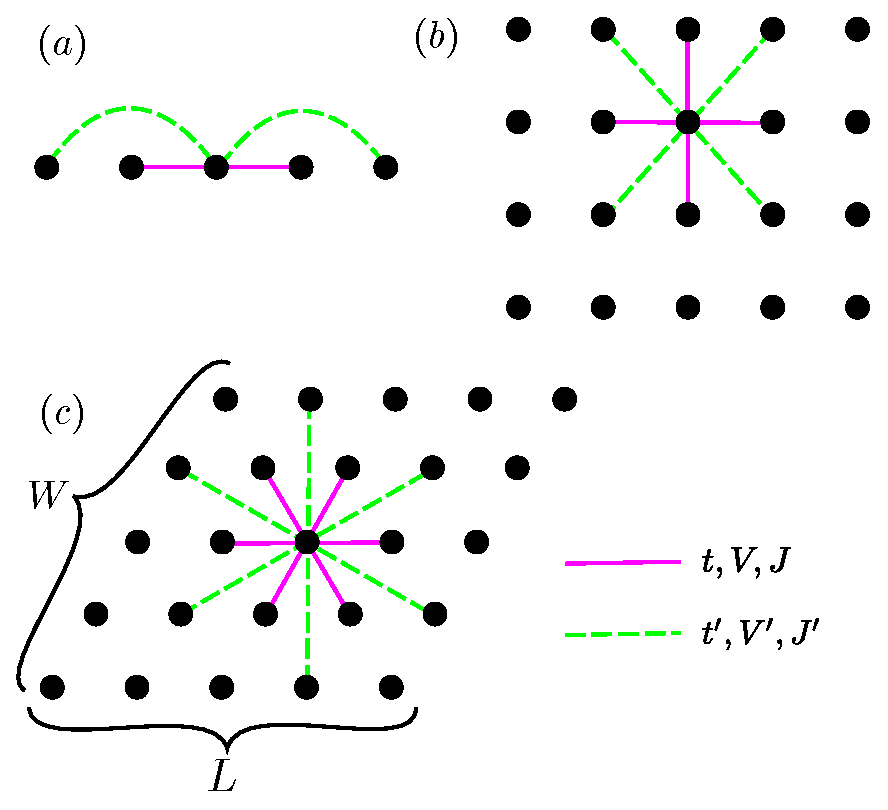
\includegraphics[width=10cm]{../figs/chap04_1_lattice.eps}
    \caption{(a)1次元鎖、(b)2次元正方格子、(c)2次元三角格子の模式図. 
      ホッピング積分、オフサイトクーロン積分、スピン結合は、
      再近接サイト間(マゼンタの実線)ではそれぞれ$t,V,J$となり、
      次近接サイト間(緑の破線)ではそれぞれ$t',V',J'$となります。}
    \label{fig_chap04_1_lattice}
  \end{center}
\end{figure}

\begin{figure}[!htbp]
  \begin{center}
    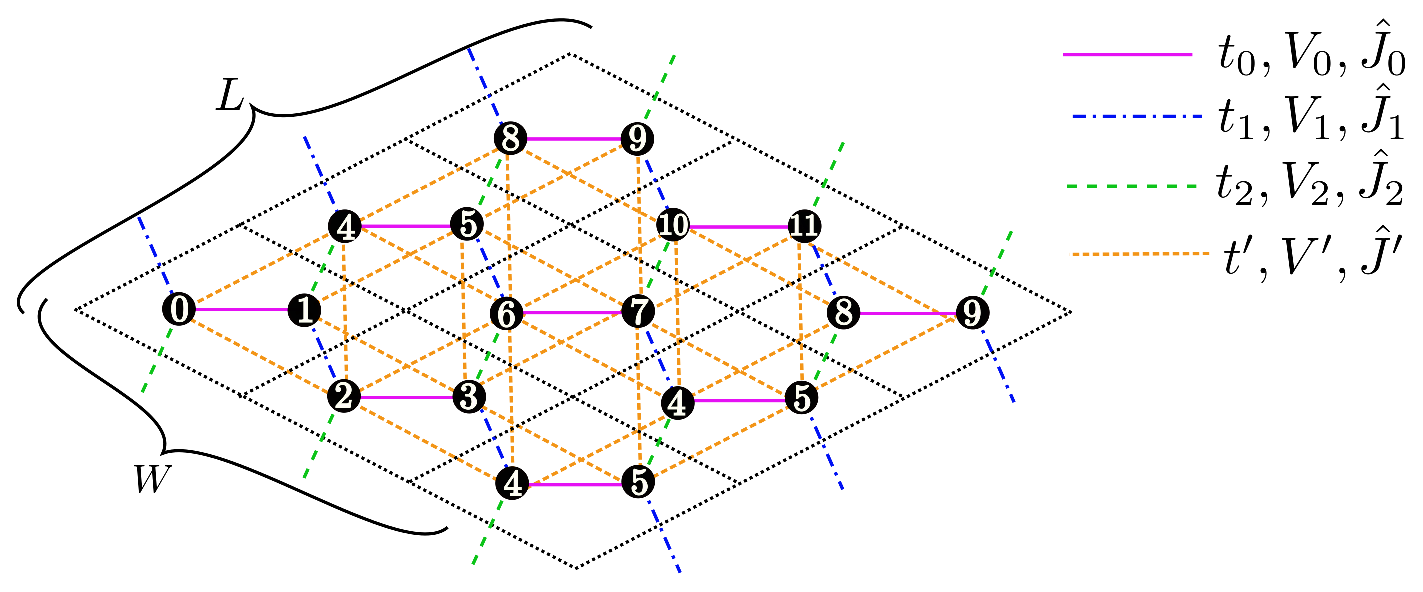
\includegraphics[width=15cm]{../figs/chap04_1_honeycomb.eps}
    \caption{2次元異方的蜂の巣格子の模式図. 
      ホッピング積分、オフサイトクーロン積分、スピン結合は、
      ボンドの方向によって異なります。
      また、次近接のホッピング積分、オフサイトクーロン積分、スピン結合
      には対応していません。
    }
    \label{fig_chap04_1_honeycomb}
  \end{center}
\end{figure}

\begin{figure}[!htbp]
  \begin{center}
    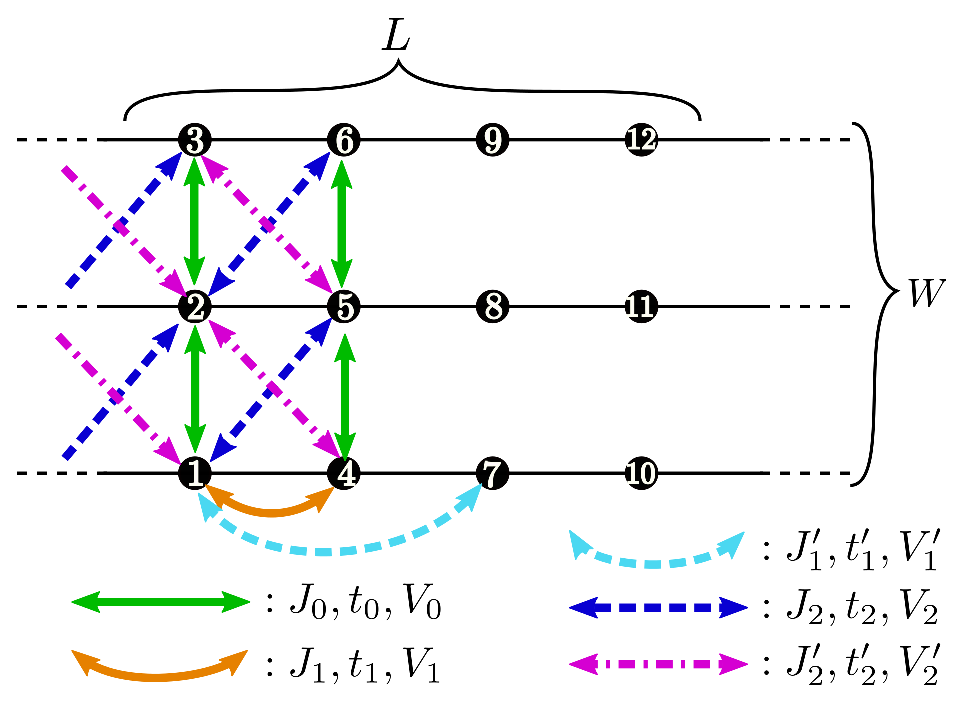
\includegraphics[width=10cm]{../figs/ladder.eps}
    \caption{梯子格子の模式図. 
    }
    \label{fig_ladder}
  \end{center}
\end{figure}

\end{itemize}

\subsection{格子に関するパラメーター}

\begin{itemize}
\item \verb|L|

{\bf 形式 :} 自然数

{\bf 説明 :} 第1次元方向の格子点数を指定します。

\item \verb|W|

{\bf 形式 :} 自然数

{\bf 説明 :} 第2次元方向の格子点数を指定します。
\verb|lattice = "Chain Lattice"|の時には使われないため、
指定をしないでください。

\item \verb|a|

{\bf 形式 :} 実数 (デフォルト値は\verb|1.0|)

{\bf 説明 :} 格子定数を指定します。
\end{itemize}

\subsection{保存量に関するパラメーター}

\begin{itemize}
\item \verb|nelec|

{\bf 形式 :} 整数

{\bf 説明 :} 伝導電子数を指定します。
\verb|lmodel = "Fermion HubbardGC"|, \verb|"Spin"|, \verb|"SpinGC"|
のときには指定しないでください。

\item \verb|2Sz|

{\bf 形式 :} 整数

{\bf 説明 :} 全スピンのz 成分の2倍を指定します。
\verb|lmodel = "Fermion HubbardGC"|, \verb|SpinGC|
のときには指定しないでください。
\end{itemize}

\subsection{Hubbard模型パラメーター}
\begin{itemize}
\item \verb|mu|

{\bf 形式 :} 実数(デフォルト値は\verb|0.0|)

{\bf 説明 :} 化学ポテンシャルを指定します。

\item \verb|t|

{\bf 形式 :} 実数(デフォルト値は\verb|1.0|)

{\bf 説明 :} 最近接サイト間のホッピング(Fig. \ref{fig_chap04_1_lattice}参照)を指定します。

\item \verb|t'|

{\bf 形式 :} 実数(デフォルト値は\verb|0.0|)

{\bf 説明 :} 次近接サイト間のホッピング(Fig. \ref{fig_chap04_1_lattice}参照)を指定します。

\item \verb|t0|, \verb|t1|, \verb|t2|

{\bf 形式 :} 実数(デフォルト値は\verb|t|)

{\bf 説明 :} 異方的蜂の巣格子での最近接サイト間のホッピング
(Fig. \ref{fig_chap04_1_honeycomb}参照)を指定します。

\item \verb|t0|, \verb|t1|, \verb|t1'|, \verb|t2|, \verb|t2'|

{\bf 形式 :} 実数(デフォルト値は\verb|1.0|)

{\bf 説明 :} 梯子格子でのホッピング
(Fig. \ref{fig_ladder}参照)を指定します。

\item \verb|U|

{\bf 形式 :} 実数(デフォルト値は\verb|0.0|)

{\bf 説明 :} オンサイトクーロン積分を指定します。

\item \verb|V|, \verb|V'|

{\bf 形式 :} 実数(デフォルト値は\verb|0.0|)

{\bf 説明 :} それぞれ最近接および次近接サイト間オフサイトクーロン積分
(Fig. \ref{fig_chap04_1_lattice}参照)を指定します。

\item \verb|V0|, \verb|V1|, \verb|V2|

{\bf 形式 :} 実数(デフォルト値は\verb|V|)

{\bf 説明 :} 異方的蜂の巣格子での最近接サイト間のオフサイトクーロン積分
(Fig. \ref{fig_chap04_1_honeycomb}参照)を指定します。

\item \verb|V0|, \verb|V1|, , \verb|V1'|, \verb|V2|, , \verb|V2'|

{\bf 形式 :} 実数(デフォルト値は\verb|0.0|)

{\bf 説明 :} 梯子格子でのオフサイトクーロン積分
(Fig. \ref{fig_ladder}参照)を指定します。

\end{itemize}

\subsection{Kitaev-Heisenberg模型パラメーター}
\begin{itemize}
\item \verb|2S|

{\bf 形式 :} 正の整数(デフォルト値は\verb|1|)

{\bf 説明 :} 局在スピンの大きさ$S$の2倍を指定します.
(例/ $1/2$スピンならば\verb|1|)

\item \verb|h|, \verb|Gamma|, \verb|D|

{\bf 形式 :} 実数(デフォルト値は\verb|0.0|)

{\bf 説明 :} それぞれ縦磁場、横磁場、異方性パラメータを指定します。

\item \verb|J|

{\bf 形式 :} 実数(デフォルト値は\verb|1.0|)

{\bf 説明 :} 最近接サイト間の等方的スピン結合(Fig. \ref{fig_chap04_1_lattice}参照)を指定します。
これが指定されていて、
\verb|Jx|, \verb|Jy|, \verb|Jz|, \verb|Jxy|のいずれも指定されていない場合には
\verb|Jx|, \verb|Jy|, \verb|Jz|, \verb|Jxy|にはすべて\verb|J|が代入されます。

\item \verb|Jz|, \verb|Jxy|

{\bf 形式 :} 実数(デフォルト値は\verb|J|)

{\bf 説明 :} 最近接サイト間の一軸性異方的スピン結合(Fig. \ref{fig_chap04_1_lattice}参照)を指定します。
\verb|Jxy|が指定されていて、
\verb|Jx|, \verb|Jy|が指定されていない場合には
\verb|Jx|, \verb|Jy|には\verb|Jxy|が代入されます。

\item \verb|Jx|, \verb|Jy|

{\bf 形式 :} 実数(デフォルト値は\verb|Jxy|)

{\bf 説明 :} 最近接サイト間の三軸性異方的スピン結合(Fig. \ref{fig_chap04_1_lattice}参照)を指定します。

\item \verb|J'|, \verb|Jx'|, \verb|Jy'|, \verb|Jz'|, \verb|Jxy'|

{\bf 形式 :} 実数(\verb|J'|のデフォルト値は\verb|0.0|, 
\verb|Jxy'|と\verb|Jz'|のデフォルト値は\verb|J'|,
\verb|Jx'|と\verb|Jy'|のデフォルト値は\verb|Jxy'|)

{\bf 説明 :} 次近接サイト間のスピン結合(Fig. \ref{fig_chap04_1_lattice}参照)を指定します。
最近接のもの(\verb|J|, \verb|Jx|, \verb|Jy|, \verb|Jz|, \verb|Jxy|)
と同様のルールで設定されます。

\item \verb|J0|, \verb|J1|, \verb|J2|, \verb|Jx0|, \verb|Jy0|, \verb|Jz0|, \verb|Jx1|, \verb|Jy1|, \verb|Jz1|, 
  \verb|Jx2|, \verb|Jy2|, \verb|Jz2|, \verb|Jxy0|, \verb|Jxy1|, \verb|Jxy2|

{\bf 形式 :} 実数 (\verb|J0|, \verb|J1|, \verb|J2|のデフォルト値は\verb|J|, 
\verb|Jxy0|, \verb|Jxy1|,  \verb|Jxy2|のデフォルト値は\verb|Jxy|
\verb|Jx0|, \verb|Jx1|, \verb|Jx2| のデフォルト値は\verb|Jx|,
\verb|Jy0|, \verb|Jy1|, \verb|Jy2| のデフォルト値は\verb|Jy|,
\verb|Jz0|, \verb|Jz1|, \verb|Jz2| のデフォルト値は\verb|Jz|)

{\bf 説明 :} 異方的蜂の巣格子の最近接サイト間のスピン結合(Fig. \ref{fig_chap04_1_honeycomb}参照)を指定します。

\item \verb|J0|, \verb|J1|, \verb|J1'|, \verb|J2|, \verb|J2'|

{\bf 形式 :} 実数 (デフォルト値は\verb|1.0|)

{\bf 説明 :} 梯子格子でのスピン結合(Fig. \ref{fig_ladder}参照)を指定します。

\end{itemize}

\subsection{近藤格子模型パラメーター}
\begin{itemize}
\item \verb|mu|

{\bf 形式 :} 実数(デフォルト値は\verb|0.0|)

{\bf 説明 :} 化学ポテンシャルを指定します。

\item \verb|t|

{\bf 形式 :} 実数(デフォルト値は\verb|1.0|)

{\bf 説明 :} 最近接サイト間のホッピング(Fig. \ref{fig_chap04_1_lattice}参照)を指定します。

\item \verb|t0|, \verb|t1|, \verb|t2|

{\bf 形式 :} 実数(デフォルト値は\verb|t|)

{\bf 説明 :} 異方的蜂の巣格子での最近接サイト間のホッピング(Fig. \ref{fig_chap04_1_honeycomb}参照)を指定します。

\item \verb|J|

{\bf 形式 :} 実数(デフォルト値は\verb|0.0|)

{\bf 説明 :} 局在電子と遍歴電子のスピン結合を指定します。
\end{itemize}

\subsection{計算条件のパラメーター}
\begin{itemize}
\item \verb|Lanczos_max|

{\bf 形式 :} 整数(デフォルト値は\verb|2000|)

{\bf 説明 :} ランチョスステップの上限を指定します。

\item \verb|initial_iv|

{\bf 形式 :} 整数(デフォルト値は\verb|1|)

{\bf 説明 :}  {初期条件のベクトルを与えます。}
\begin{itemize}
\item{ランチョス法}
\begin{itemize}
\item{カノニカル集団かつ \verb|initial_iv| $\geq 0$の場合}

ノンゼロの成分が指定されます。

\item{ \verb|initial_iv| $< 0$の場合}

乱数のシードが指定され、全ての成分に対して係数がランダムに与えられます。なお、グランドカノニカルの場合は初期状態として多くの状態を持つよう、こちらの様式が適用されます。
\end{itemize}

\item{TPQ法}

乱数のシードが指定され、全ての成分に対して係数がランダムに与えられます。
\end{itemize}
初期ベクトル設定の詳細については、\ref{Ch:algorithm}を参照ください。

\item \verb|nvec|

{\bf 形式 :} 整数(デフォルト値は\verb|1|)

{\bf 説明 :} ランチョス法の段階で下からいくつの固有値を求めるかを指定します。

\item \verb|exct|

{\bf 形式 :} 整数(デフォルト値は\verb|1|)

{\bf 説明 :} エネルギーの低いものから数えて、何番目の固有状態を計算するかを指定します。

\item \verb|LanczosEps|

{\bf 形式 :} 整数(デフォルト値は\verb|14|)

{\bf 説明 :} ランチョスの収束判定条件を指定します。
ひとつ前のステップの固有値との相対誤差が, $10^{-{\tt LanczosEps}}$以下になったら収束したと判断します。

\item \verb|LancczosTarget|

{\bf 形式 :} 整数(デフォルト値は\verb|2|)

{\bf 説明 :} エネルギーの低いものから数えて、
何番目の固有値でランチョスの収束判定を行うかを指定します。

\item \verb|LargeValue|

{\bf 形式 :} 実数(デフォルト値は下記参照)

{\bf 説明 :} (TPQ法のみで使用)$l-\hat{H}/N_{s}$の$l$。各模型、格子ごとにデフォルト値が次のように変わります。

\begin{itemize}

\item Hubbard模型[式(\ref{fml4_1_hubbard})]

カノニカル集団
\begin{align}
l = |\mu| \frac{N_{\rm elec}}{N_{\rm site}}
+ 2 z |t| + 2 z' |t'| + |U| + 2 z |V| + 2 z' |V'| 
\end{align}
グランドカノニカル集団
\begin{align}
l = 2|\mu|
+ 2 z |t| + 2 z' |t'| + |U| + 2 z |V| + 2 z' |V'|
\end{align}

\item Kitaev-Heisenberg模型[式(\ref{fml4_1_spin})]

カノニカル集団
\begin{align}
l = \frac{|S_z^{\rm tot}|}{N_{\rm site}}|h| + S |\Gamma| + S^2 |D|
+\frac{z}{2} S^2 (|J_x|+|J_y|+|J_z|) +\frac{z'}{2} S^2 (|J'_x|+|J'_y|+|J'_z|)
\end{align}
グランドカノニカル集団
\begin{align}
l = S |h| + S |\Gamma| + S^2 |D|
+\frac{z}{2} S^2 (|J_x|+|J_y|+|J_z|) + \frac{z'}{2} S^2 (|J'_x|+|J'_y|+|J'_z|) 
\end{align}

\item 近藤格子模型[式(\ref{fml4_1_kondo})]

カノニカル集団
\begin{align}
l = |\mu| \frac{N_{\rm elec}}{N_{\rm site}} + 2 z |t| + \frac{S}{2} |J| 
\end{align}
グランドカノニカル集団
\begin{align}
l = 2|\mu| + 2 z |t| + \frac{S}{2} |J| 
\end{align}

\end{itemize}

\item \verb|NumAve|

{\bf 形式 :} 整数(デフォルト値は\verb|5|)

{\bf 説明 :} (TPQ法のみで使用)独立なrunを何回行うかを指定します。

\item \verb|ExpecInterval|

{\bf 形式 :} 整数(デフォルト値は\verb|20|)

{\bf 説明 :} (TPQ法のみで使用)相関関数の計算を何回のTPQステップおきに行うかの指定。
頻度を上げると計算コストが増大するので注意してください。
\end{itemize}

